\newpage
\section{Diagrammi delle attività}
Vengono illustrati ora i diagrammi di attività. Viene illustrato il diagramma principale ad alto livello e i diversi sotto-diagrammi specifici.

\subsection{Attività principali}

\begin{figure}[h!]
		\centering
		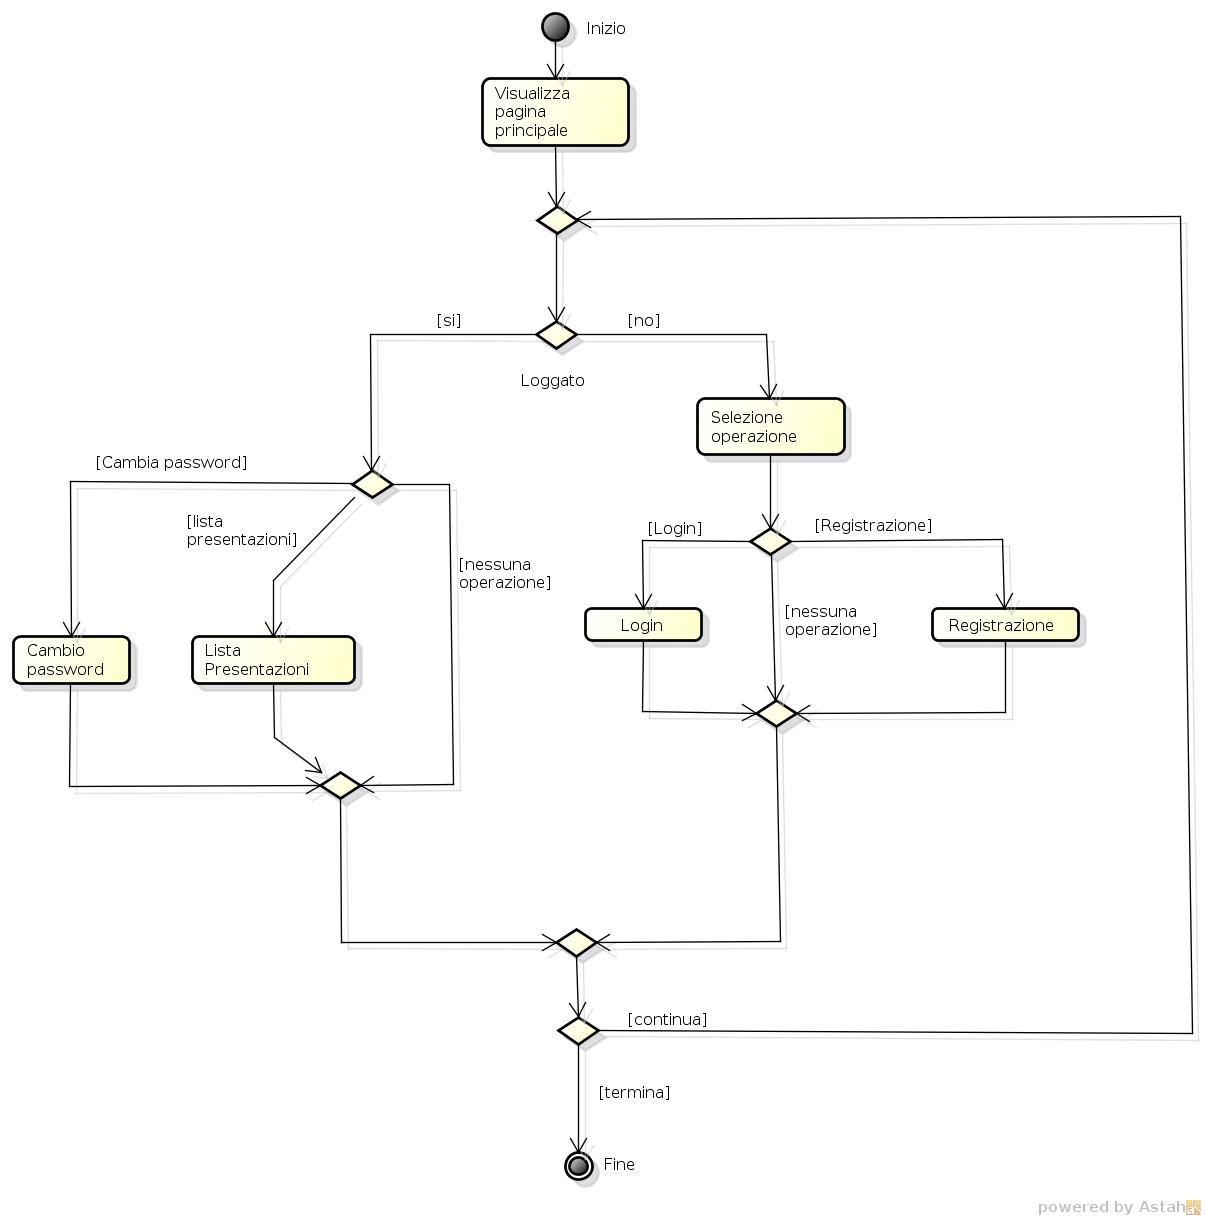
\includegraphics[scale=.4]{img/Premi.jpg}
		\caption{Attività principali}
		\label{fig:Attivita_principali}
\end{figure}

L'utente nel momento in cui accede nel programma ha la possibilità di effettuare la login o di registrarsi nel sistema. 
L'utente loggato può invece effettuare il logout, andare nella lista presentazioni ed effettuare il cambio password.

\subsection{Lista presentazioni}

\begin{figure}[h!]
		\centering
		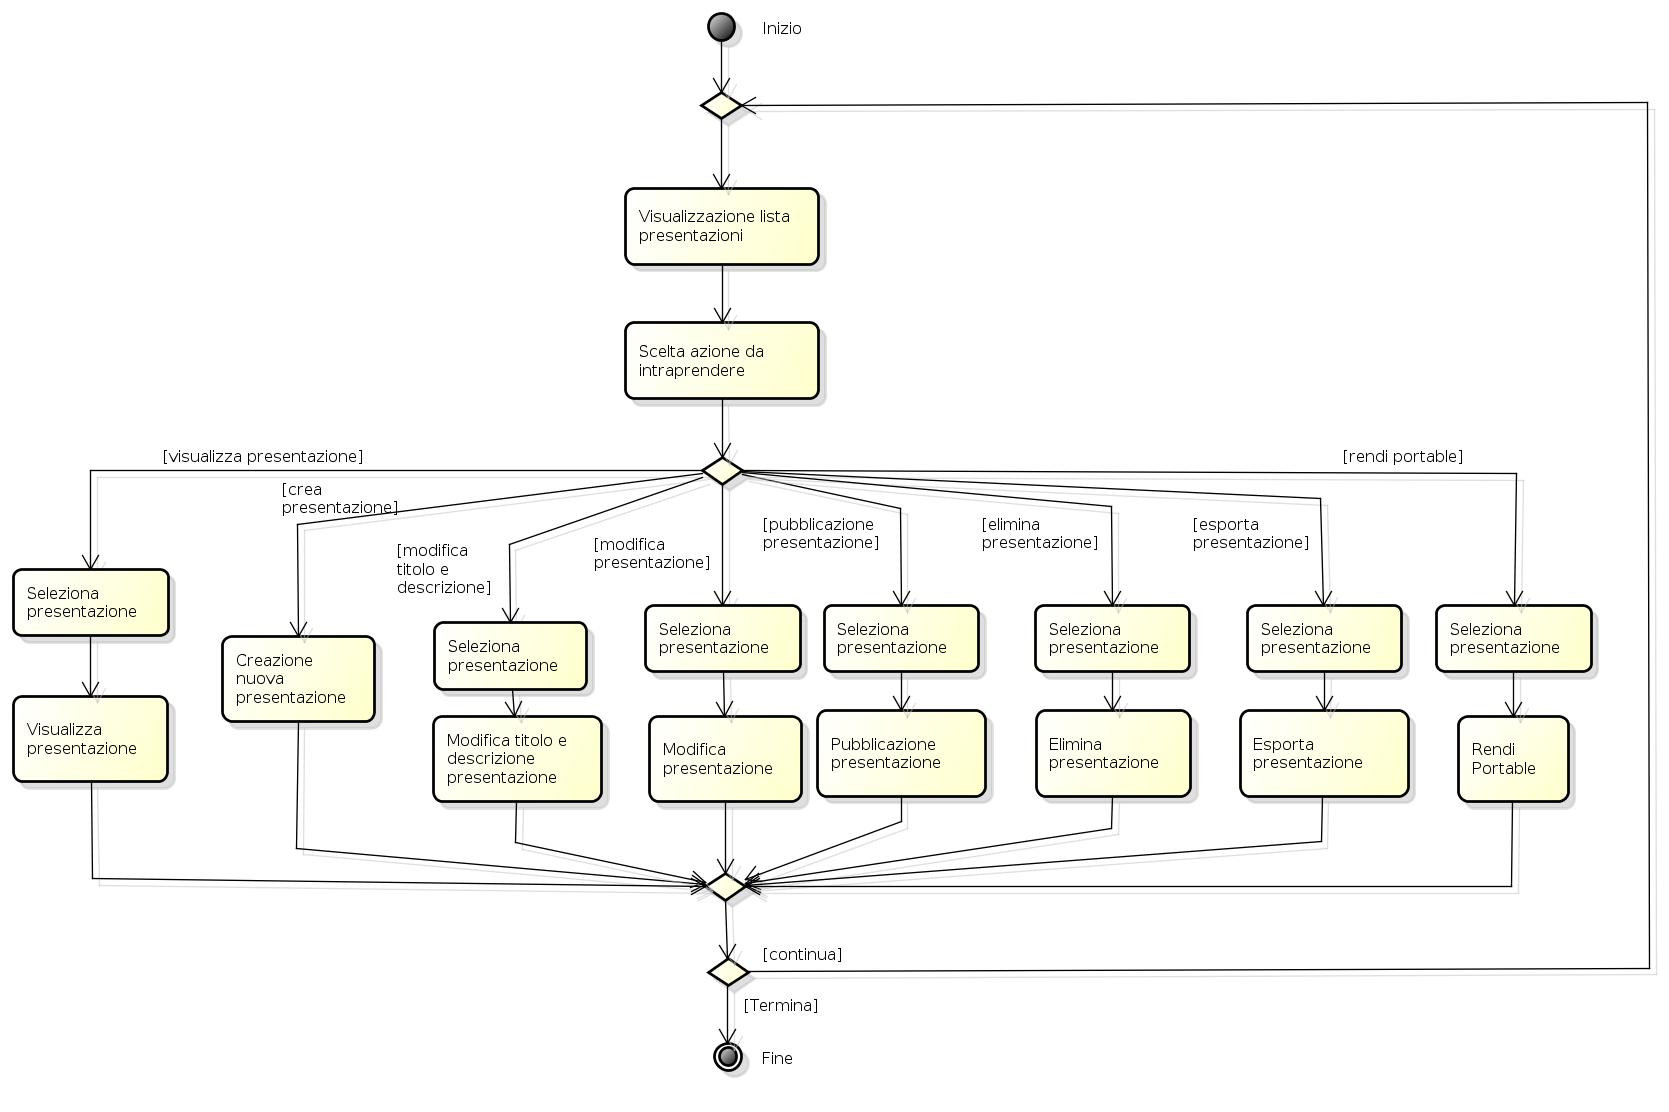
\includegraphics[scale=.35]{img/ListaPresentazioni.jpg}
		\caption{Lista presentazioni}
		\label{fig:Lista_presentazioni}
\end{figure}

\clearpage

Le scelte che ha l'utente una volta entrato nella lista presentazioni sono: Visualizza presentazione, creazione nuova presentazione, modifica titolo e descrizione presentazione, modifica presentazione, pubblicazione presentazione, elimina presentazione, esporta presentazione, rendi portable.

\subsection{Login}

\begin{figure}[h!]
		\centering
		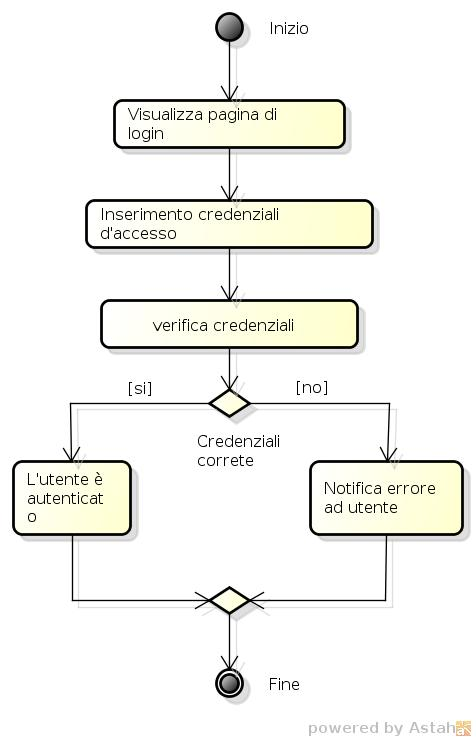
\includegraphics[scale=.5]{img/Login.jpg}
		\caption{Login utente}
		\label{fig:Login}
\end{figure}

L'utente quando accede nella pagina di login inserisce le credenziali che corrispondono a email e password. Se sono corrette viene autenticato altrimenti viene restituito un messaggio d'errore.

\newpage

\subsection{Registrazione}

\begin{figure}[h!]
		\centering
		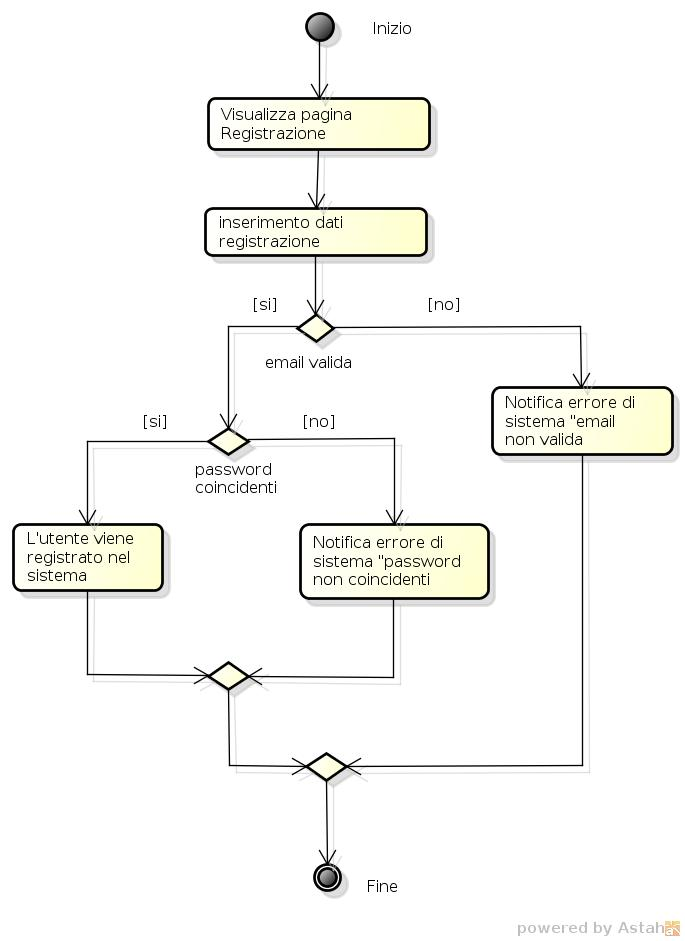
\includegraphics[scale=.5]{img/Registrazione.jpg}
		\caption{Registrazione utente}
		\label{fig:Registrazione}
\end{figure}

L'utente quando accede nella parte di registrazione inserisce l'email e la password. Se l'email non ha un formato valido o se è già presente nel sistema viene restituito un errore altrimenti viene verificato che le password inserite coincidano. In caso affermativo l'utente viene registrato nel sistema, altrimenti viene restituito un messaggio d'errore.

\newpage

\subsection{Cambio password}

\begin{figure}[h!]
		\centering
		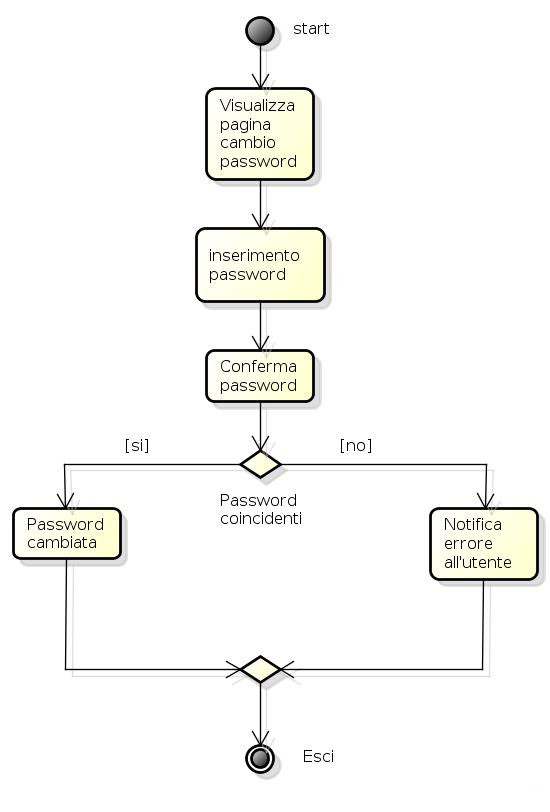
\includegraphics[scale=.5]{img/Cambio_password.jpg}
		\caption{Cambio password}
		\label{fig:Cambio_password}
\end{figure}

Per effettuare il cambio password l'utente inserisce la nuova password e la conferma della nuova. Se sono coincidenti viene effettuato il cambio password altrimenti viene notificato un errore all'utente.

\newpage

\subsection{Visualizzatore}

\begin{figure}[h!]
		\centering
		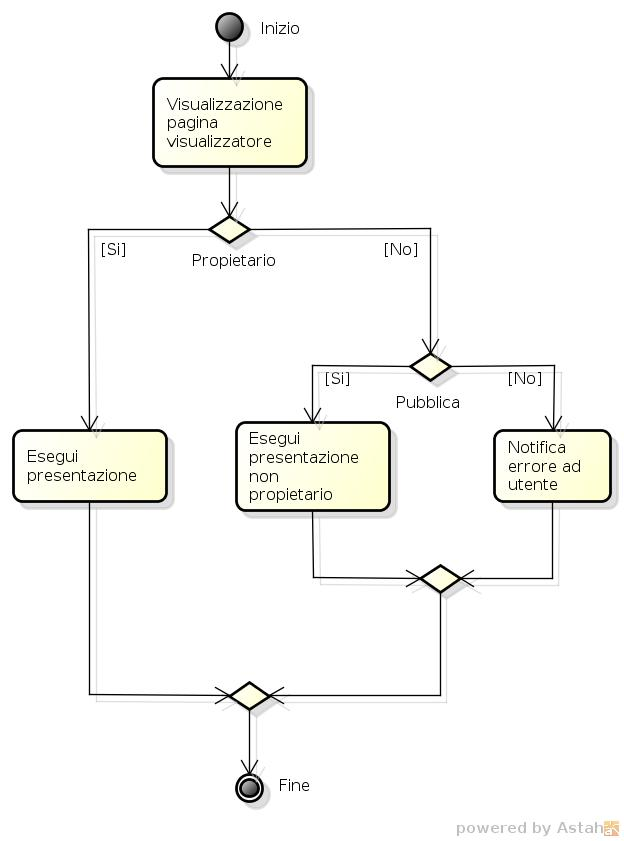
\includegraphics[scale=.5]{img/Visualizzatore.jpg}
		\caption{Visualizzatore}
		\label{fig:Visualizzatore}
\end{figure} 

Se l'utente che visualizza la presentazione è l'utente proprietario viene eseguita la presentazione in modalità proprietario altrimenti viene controllato se la presentazione è pubblica. In caso affermativo viene eseguita la presentazione in modalità non proprietario altrimenti viene notificato un errore, in quanto se la presentazione non è pubblica non può essere visualizzata. L'utente non proprietario per accedere ad una presentazione deve ottenere il link generato dall'utente proprietario nel momento in cui la rende pubblica. L'utente proprietario può rendere privata una presentazione in ogni momento perciò il controllo se è pubblica, deve essere effettuato per controllare se il link è ancora valido.

\newpage

\subsection{Esegui presentazione proprietario}

\begin{figure}[h!]
		\centering
		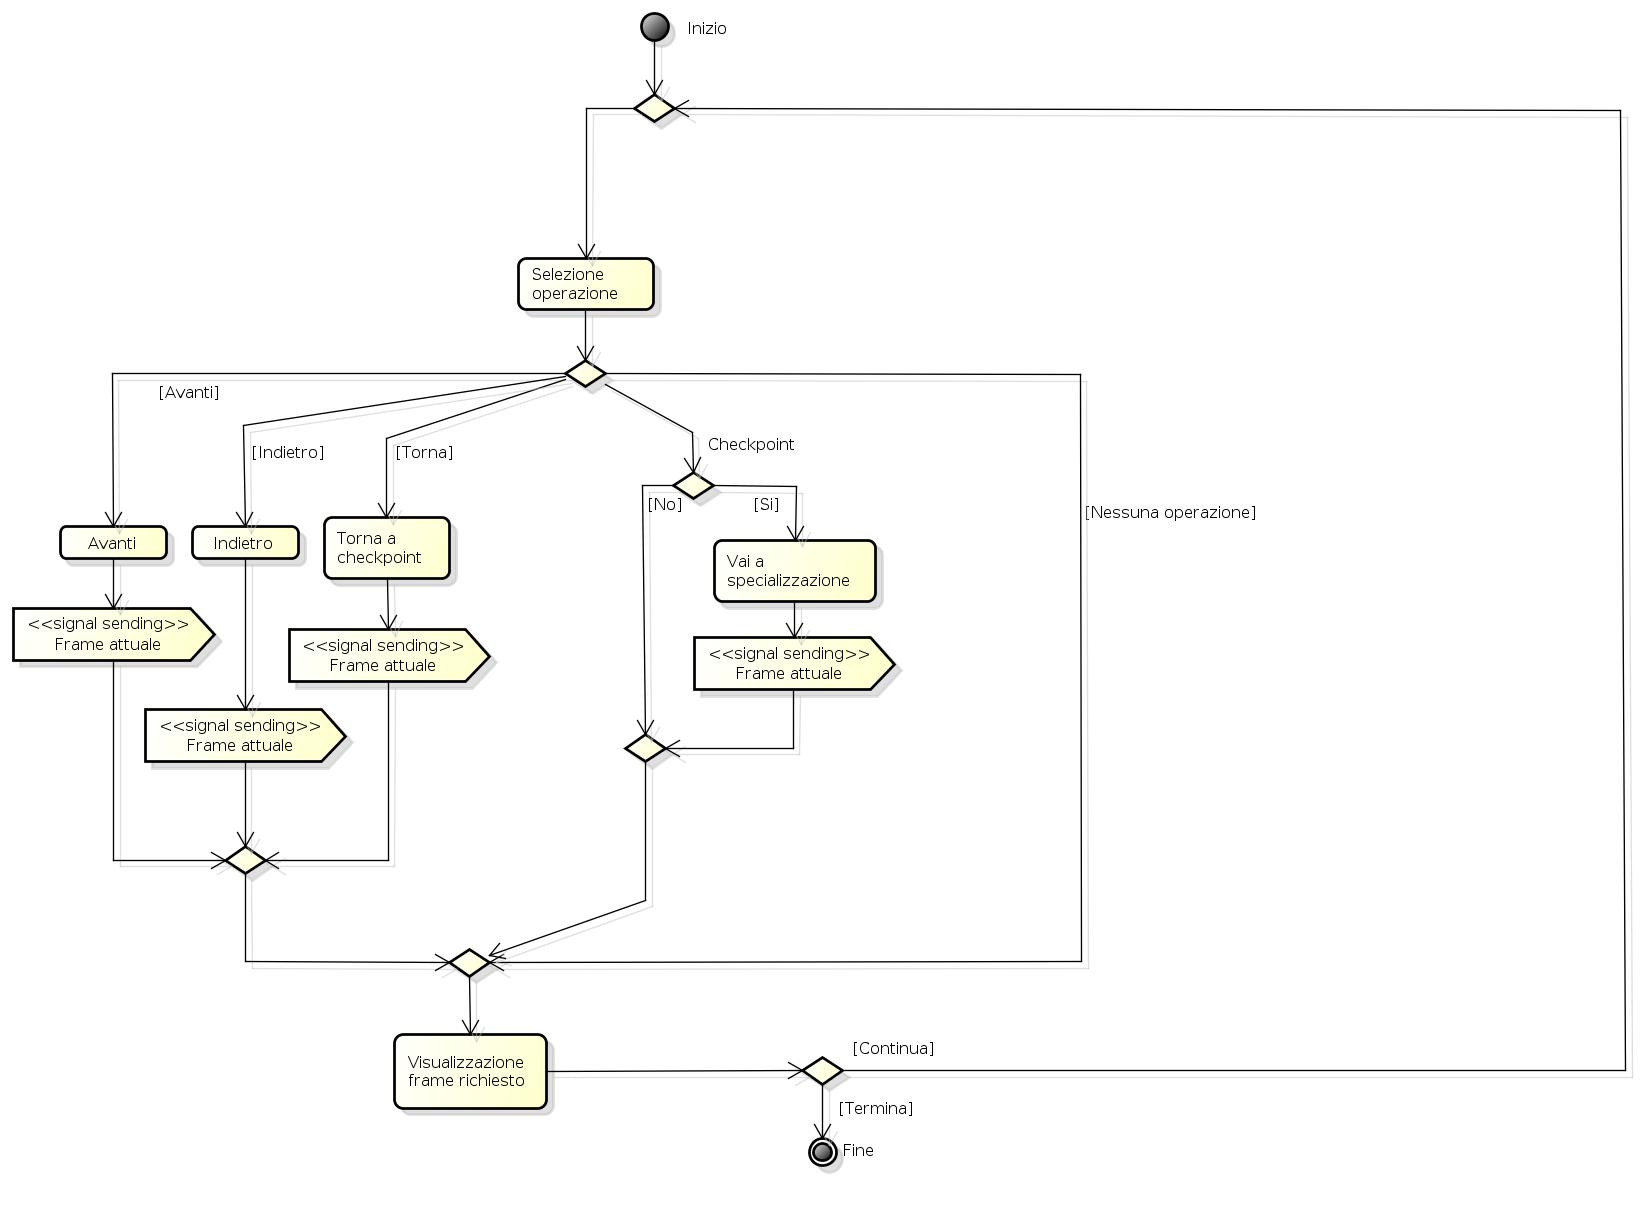
\includegraphics[scale=.4]{img/Esegui_presentazione_proprietario.jpg}
		\caption{Esegui presentazione proprietario}
		\label{fig:Esegui_presentazione_proprietario}
\end{figure}

Se la modalità di visualizzazione presentazione è in modalità proprietario si hanno le seguenti scelte: 
\begin{itemize}
\item
avanti: per andare avanti di una frame; 
\item 
indietro: per tornare indietro di un frame;
\item torna a checkpoint: permette di tornare al frame iniziale o di tornare al checkpoint se si è entrati in un percorso di specializzazione; 
\item checkpoint: se il frame corrente è un checkpoint l'utente con questa scelta entra nel percorso di specializzazione.
\end{itemize}
Il segnale Frame attuale inviato permette agli utenti non proprietari di visualizzare il frame corrente scelto dal proprietario.
L'utente ha la possibilità di uscire quando lo desidera.

\newpage

\subsection{Esegui presentazione non proprietario}

\begin{figure}[h!]
		\centering
		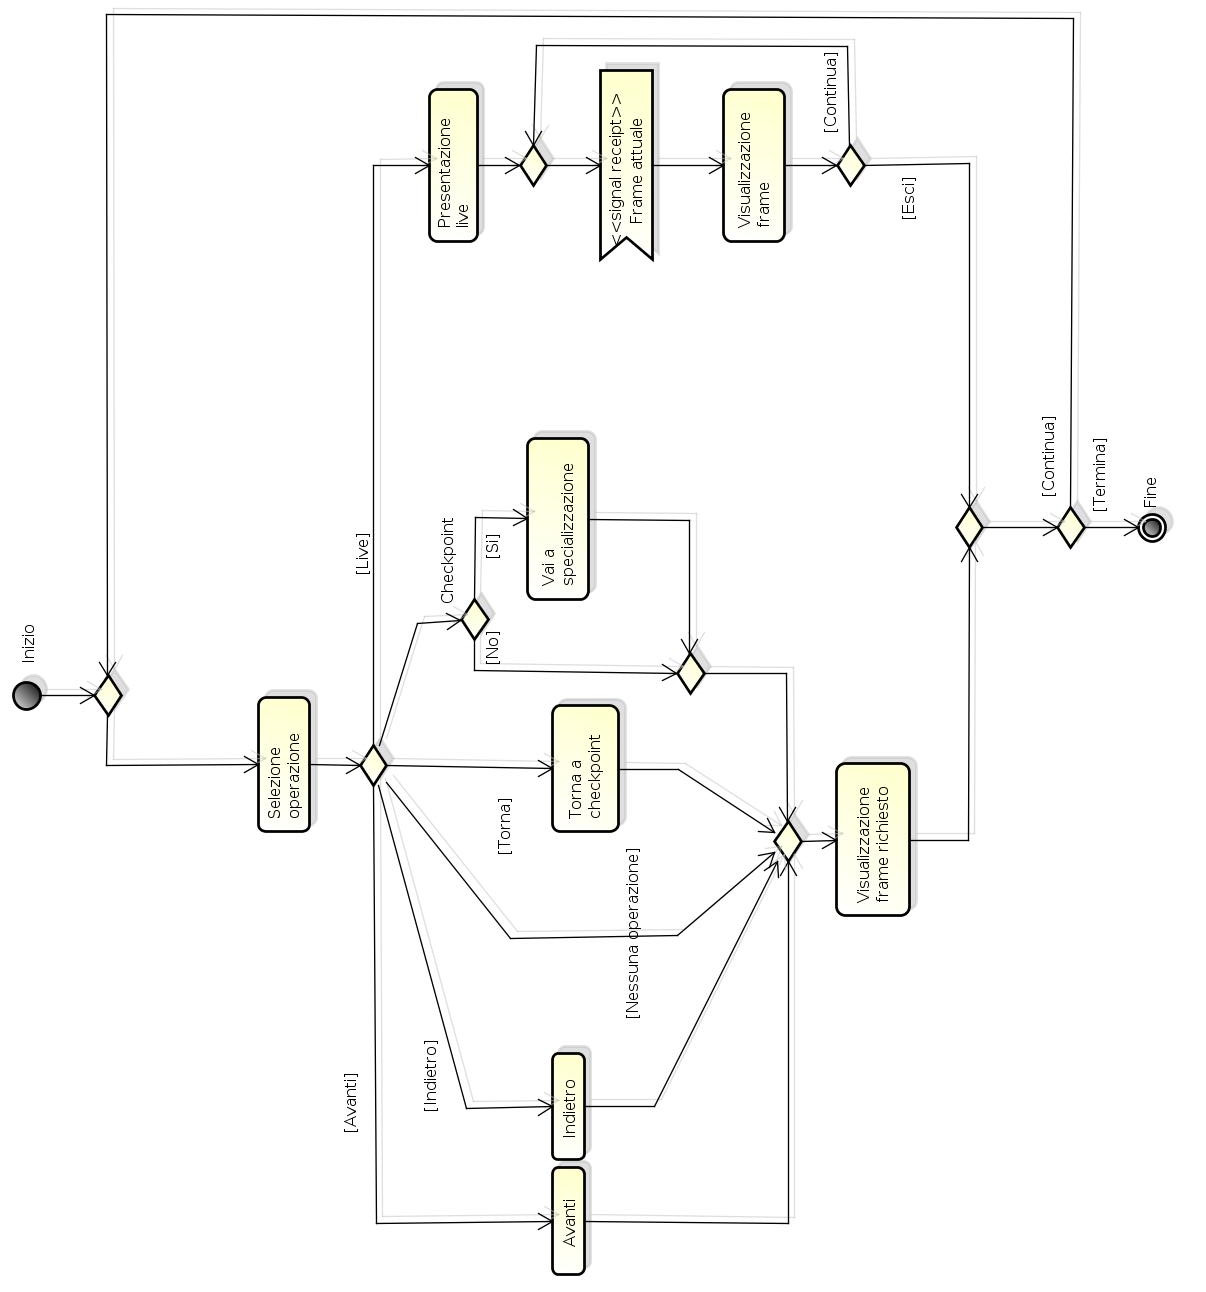
\includegraphics[scale=.4]{img/Esegui_presentazione_non_proprietario.jpg}
		\caption{Esegui presentazione non proprietario}		\label{fig:Esegui_presentazione_non_proprietario}
\end{figure}

Se la modalità di visualizzazione presentazione è in modalità proprietario si hanno le seguenti scelte: 
\begin{itemize}
\item
avanti: per andare avanti di una frame; 
\item 
indietro: per tornare indietro di un frame;
\item torna a checkpoint: permette di tornare al frame iniziale o di tornare al checkpoint se si è entrati in un percorso di specializzazione; 
\item checkpoint: se il frame corrente è un checkpoint l'utente con questa scelta entra nel percorso di specializzazione;
\item presentazione live: con questa scelta l'utente visualizza il frame corrente che l'utente proprietario ha scelto di visualizzare.
\end{itemize}
L'utente ha la possibilità di uscire quando lo desidera.

\subsection{Creazione presentazione}

\begin{figure}[h!]
		\centering
		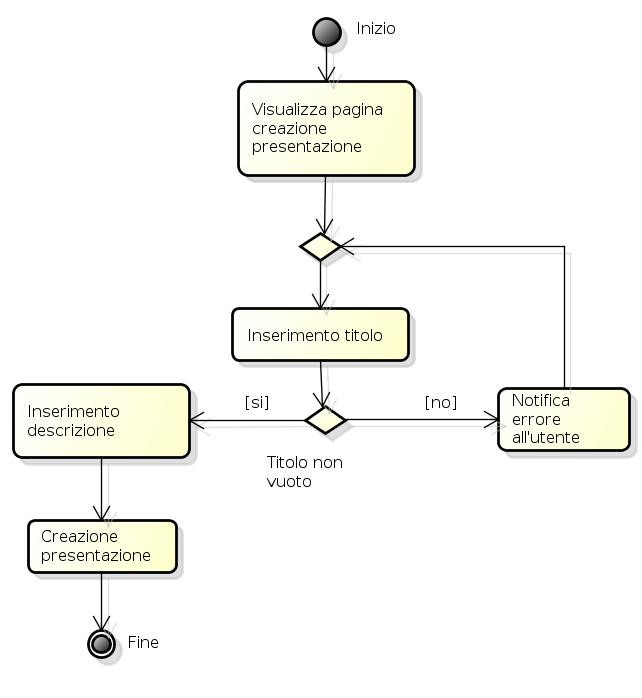
\includegraphics[scale=.5]{img/Creazione_presentazione.jpg}
		\caption{Creazione presentazione}
		\label{fig:Creazione_presentazione}
\end{figure}

L'utente può creare una nuova presentazione inserendo titolo e descrizione. Se non inserisce il titolo viene visualizzata una notifica di errore altrimenti la presentazione viene inserita nel sistema.

\newpage

\subsection{Modifica titolo e descrizione presentazione}

\begin{figure}[h!]
		\centering
		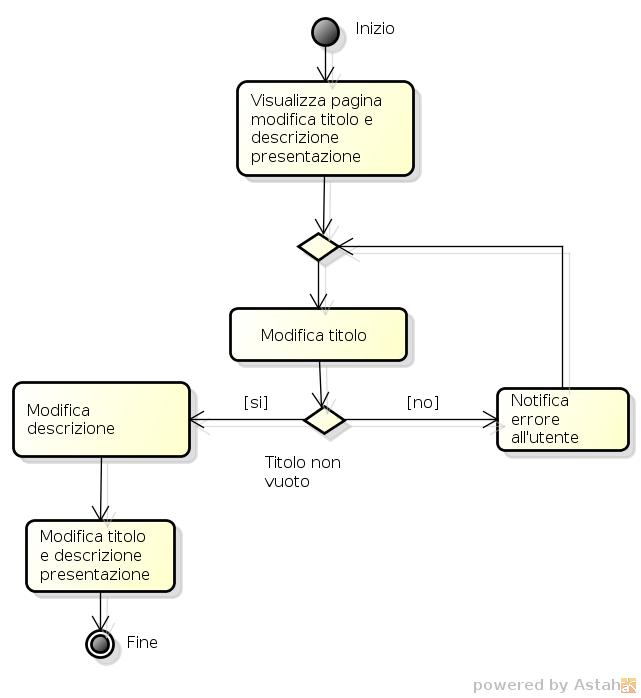
\includegraphics[scale=.5]{img/Modifica_titolo_e_descrizione_presentazione.jpg}
		\caption{Modifica titolo e descrizione della presentazione}		\label{fig:Modifica_titolo_e_descrizione_presentazione}
\end{figure}

L'utente può modificare sia il titolo che la descrizione. Se il titolo non è vuoto le modifiche vengono salvate altrimenti viene restituita una notifica di errore.

\newpage

\subsection{Pubblicazione presentazione}

\begin{figure}[h!]
		\centering
		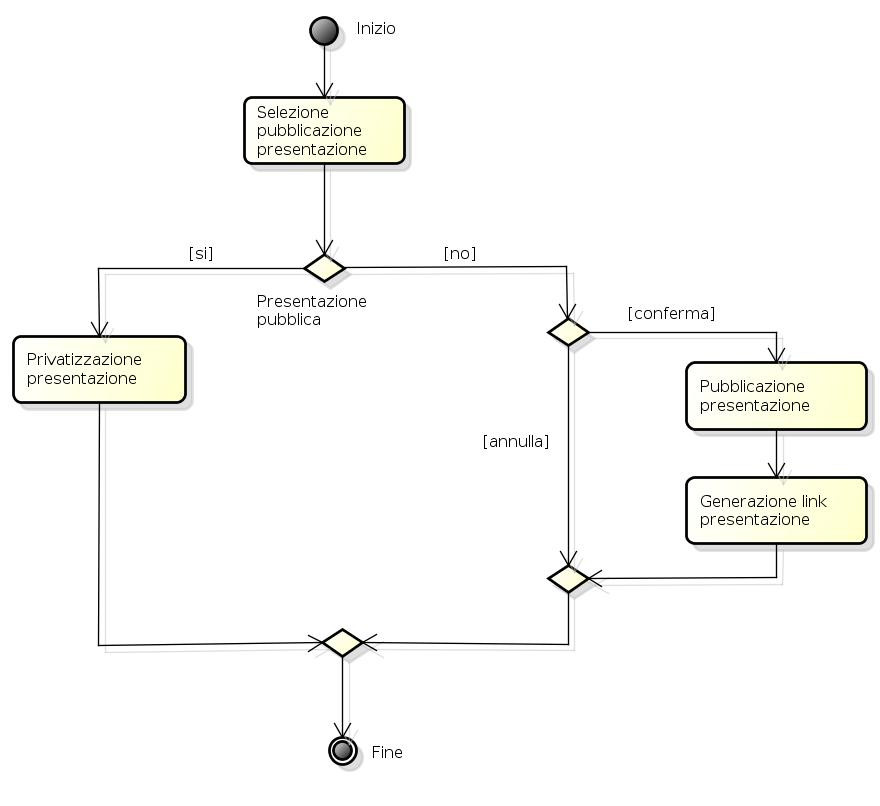
\includegraphics[scale=.5]{img/Pubblica_presentazione.jpg}
		\caption{Pubblicazione presentazione}
		\label{fig:Pubblicazione_presentazione}
\end{figure}

Se la presentazione è già pubblica rende privata la stessa, altrimenti se conferma la pubblicazione la rende visibile al pubblico e viene generato un link da inviare a chi voglia visualizzarla.

\newpage

\subsection{Elimina presentazione}

\begin{figure}[h!]
		\centering
		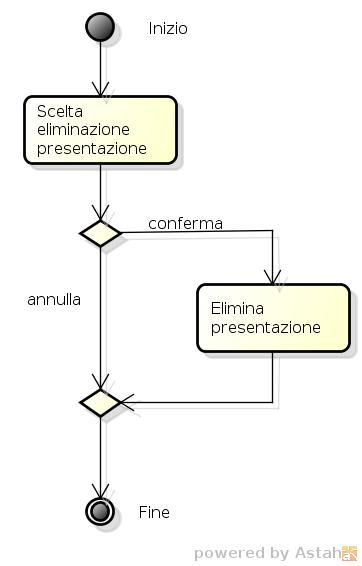
\includegraphics[scale=.5]{img/Elimina_presentazione.jpg}
		\caption{Elimina presentazione}
		\label{fig:Elimina_presentazione}
\end{figure}  

L'utente deve confermare l'eliminazione altrimenti l'operazione viene annullata.

\newpage

\subsection{Esportazione presentazione}

\begin{figure}[h!]
		\centering
		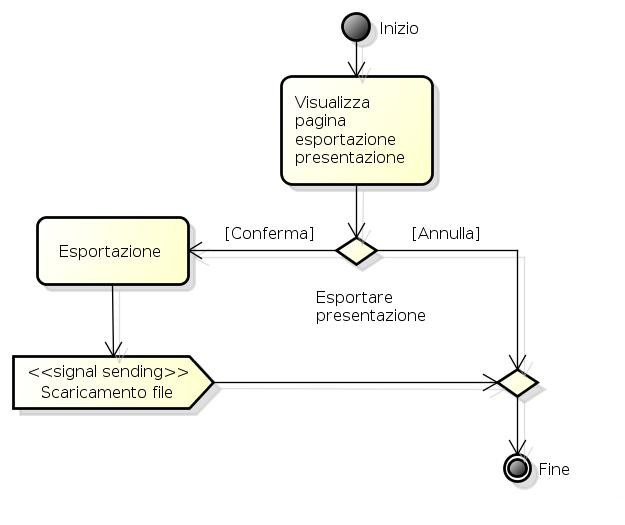
\includegraphics[scale=.5]{img/Esporta_presentazione.jpg}
		\caption{Esportazione presentazione}
		\label{fig:Esportazione_presentazione}
\end{figure}

L'utente può esportare la presentazione in modo da ottenere un poster. Se l'operazione è confermata vengono esportati i dati e si procede allo scaricamento del file. Altrimenti viene annullata.

\newpage

\subsection{Rendi portable}

\begin{figure}[h!]
		\centering
		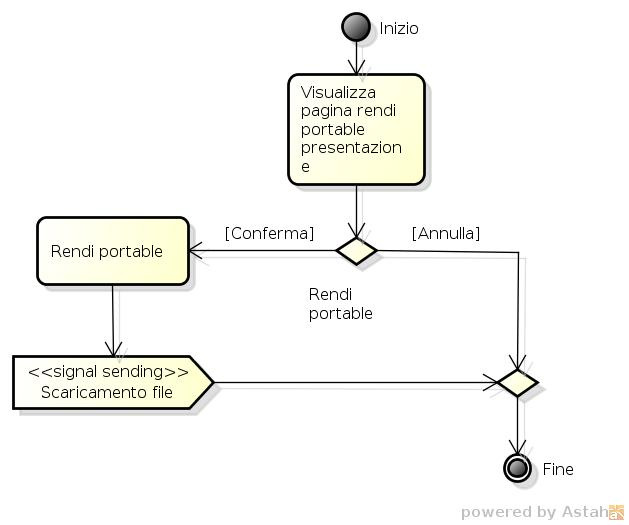
\includegraphics[scale=.5]{img/Rendi_portable.jpg}
		\caption{Rendi portable}
		\label{fig:Rendi_portable}
\end{figure}

L'utente può rendere portabile la presentazione in modo da vederla offline. Se l'operazione è confermata la presentazione viene resa portabile e si procede allo scaricamento dei file. Altrimenti viene annullata.

\newpage

\subsection{Modifica presentazione}

\begin{figure}[h!]
		\centering
		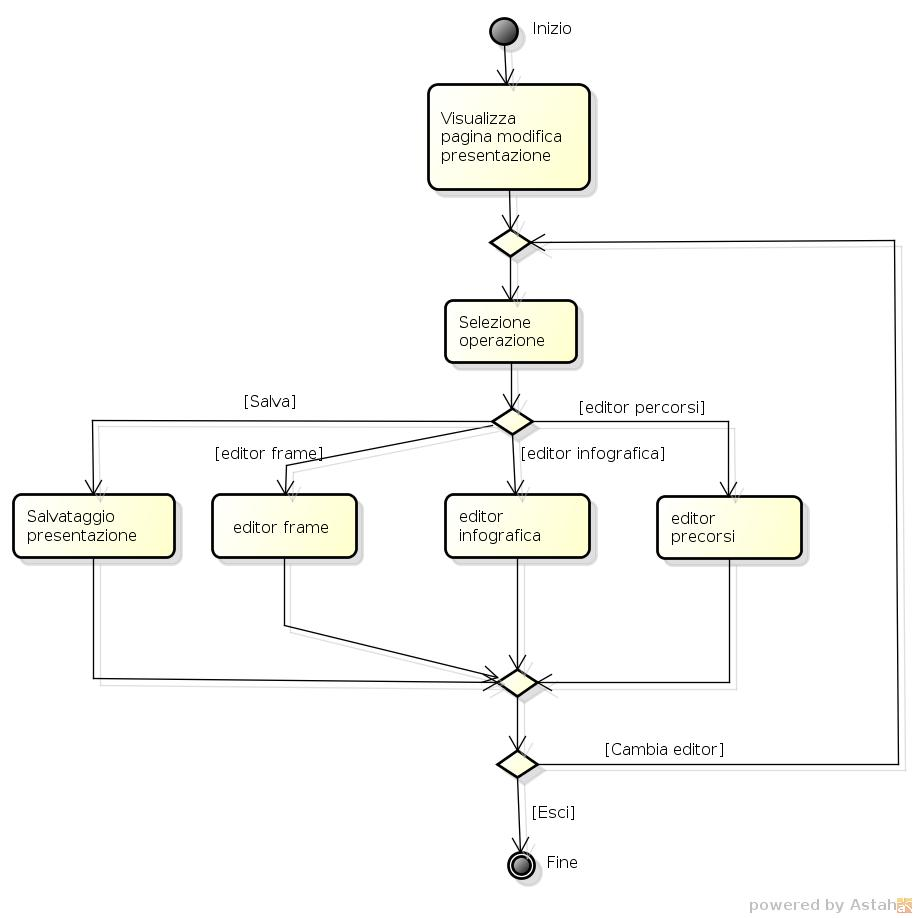
\includegraphics[scale=.5]{img/Modifica_presentazione.jpg}
		\caption{Modifica presentazione}
		\label{fig:Modifica_presentazione}
\end{figure}

L'utente può scegliere di: salvare la presentazione, andare nel frame editor, andare nell'infografica editor o nell'editor percorsi.
L'utente può in ogni momento cambiare editor.

\newpage

\subsection{Frame editor}

\begin{figure}[h!]
		\centering
		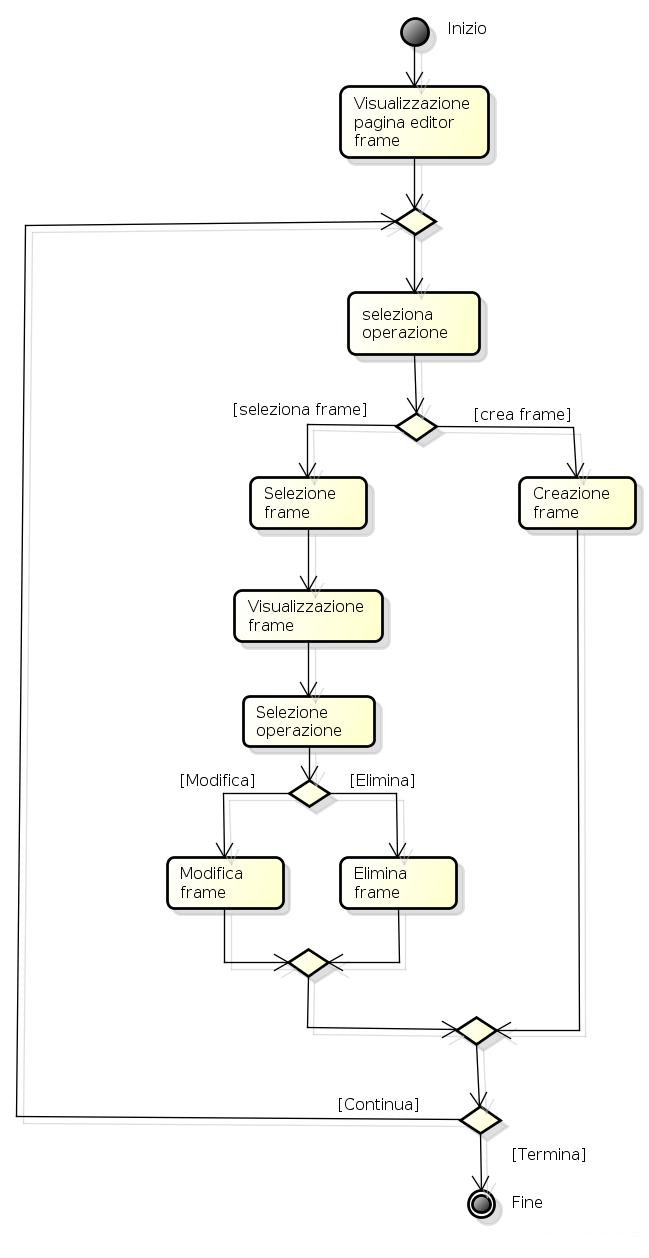
\includegraphics[scale=.5]{img/Editor_frame.jpg}
		\caption{Frame editor}
		\label{fig:Frame_editor}
\end{figure}

L'utente procede alla creazione del frame oppure può selezionarne uno. Una volta selezionato viene visualizzato nell'editor e a questo punto può scegliere se eliminarlo o modificarlo.

\newpage

\subsection{Modifica frame}

\begin{figure}[h!]
		\centering
		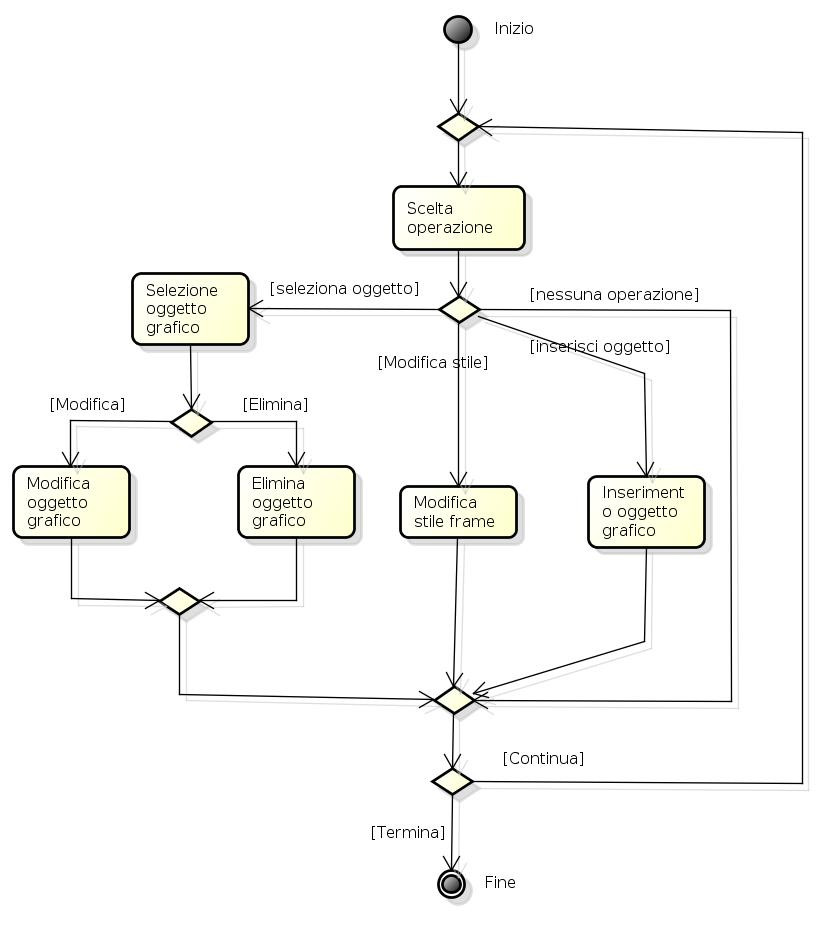
\includegraphics[scale=.5]{img/Modifica_frame.jpg}
		\caption{Modifica frame}
		\label{fig:Modifica_frame}
\end{figure}

L'utente può effettuare le seguenti operazioni:
\begin{itemize}
\item Selezione oggetto grafico: una volta selezionato l'oggetto può essere eliminato o modificato;
\item Modificare lo stile del frame;
\item Inserire un oggetto grafico nel frame;
\item Non effettuare nessuna operazione.
\end{itemize}

\newpage

\subsection{Infografica editor}

\begin{figure}[h!]
		\centering
		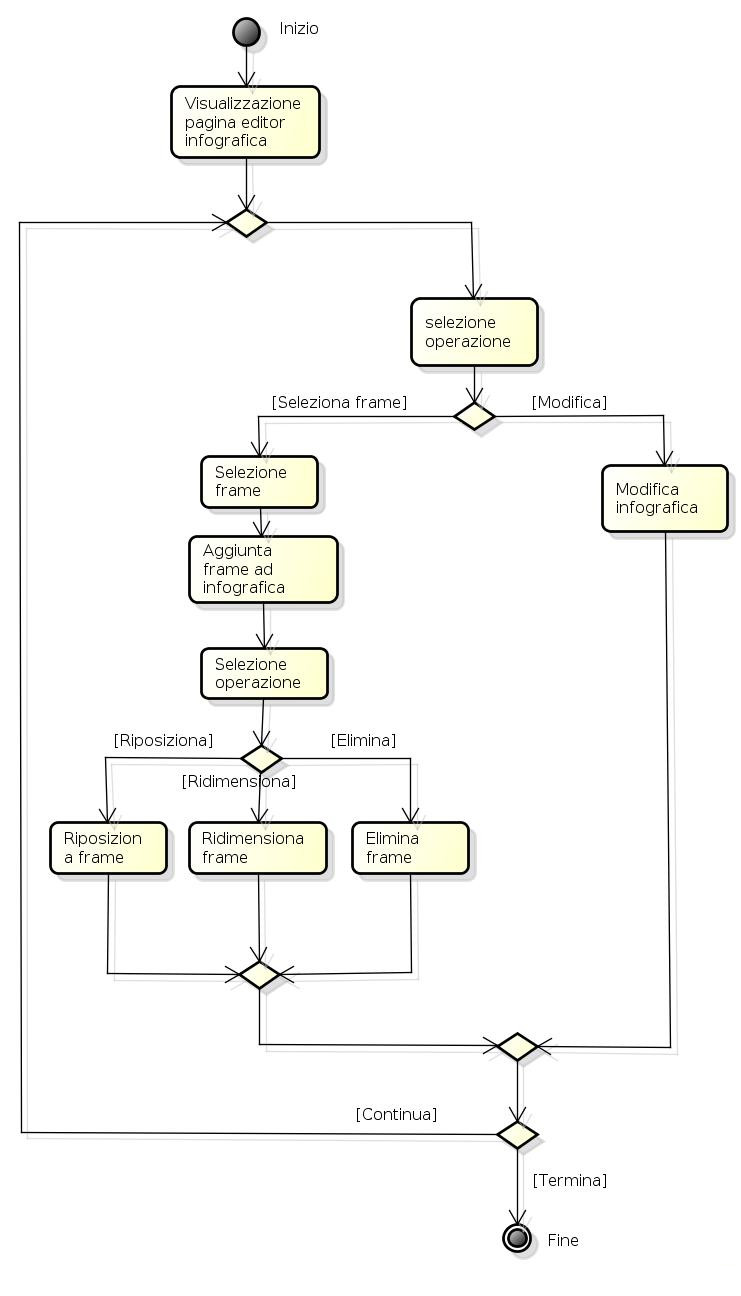
\includegraphics[scale=.4]{img/Editor_infografica.jpg}
		\caption{Infographic editor}
		\label{fig:Infografica_editor}
\end{figure}

L'utente può scegliere di: 
\begin{itemize}
\item modificare l'infografica 
\item selezionare un frame e successivamente aggiungierlo all'infografica, eliminarlo dall'infografica o cambiargli la posizione e la grandezza e altezza.
\end{itemize}

\newpage

\subsection{Modifica infografica}

\begin{figure}[h!]
		\centering
		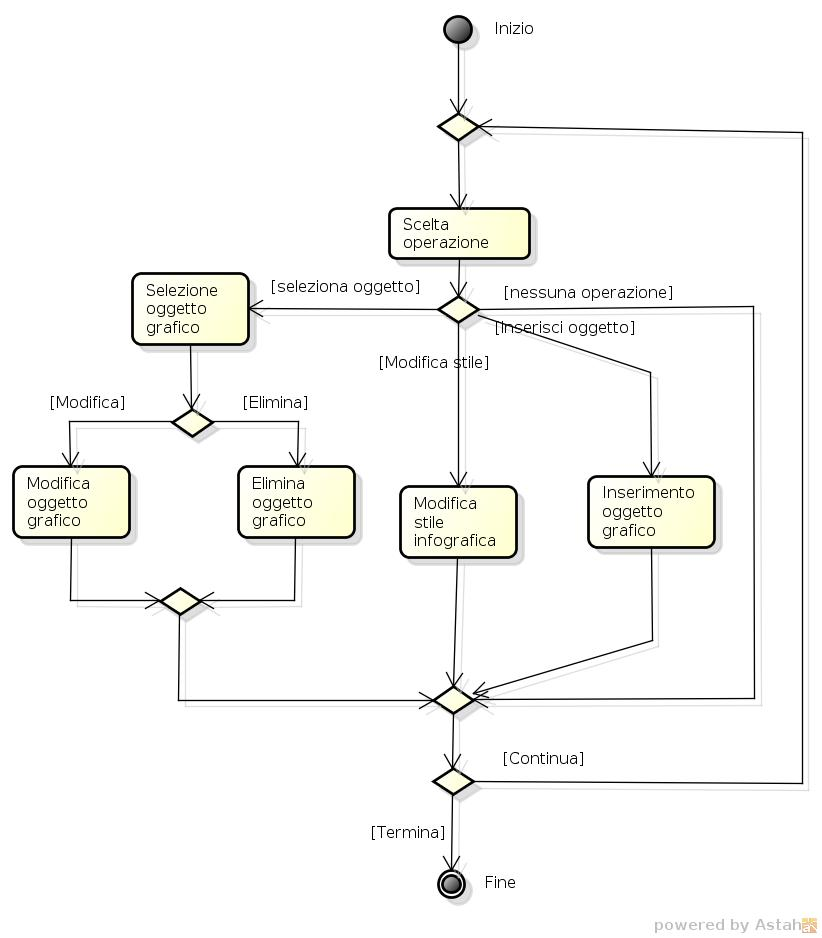
\includegraphics[scale=.5]{img/Modifica_infografica.jpg}
		\caption{Modifica infografica}
		\label{fig:Modifica_infografica}
\end{figure}

L'utente può effettuare le seguenti operazioni:
\begin{itemize}
\item Selezione oggetto grafico: una volta selezionato l'oggetto può essere eliminato o modificato;
\item Modificare lo stile dell'infografica;
\item Inserire un oggetto grafico nell'infografica;
\item Non effettuare nessuna operazione.
\end{itemize}

\newpage

\subsection{Editor percorsi}

\begin{figure}[h!]
		\centering
		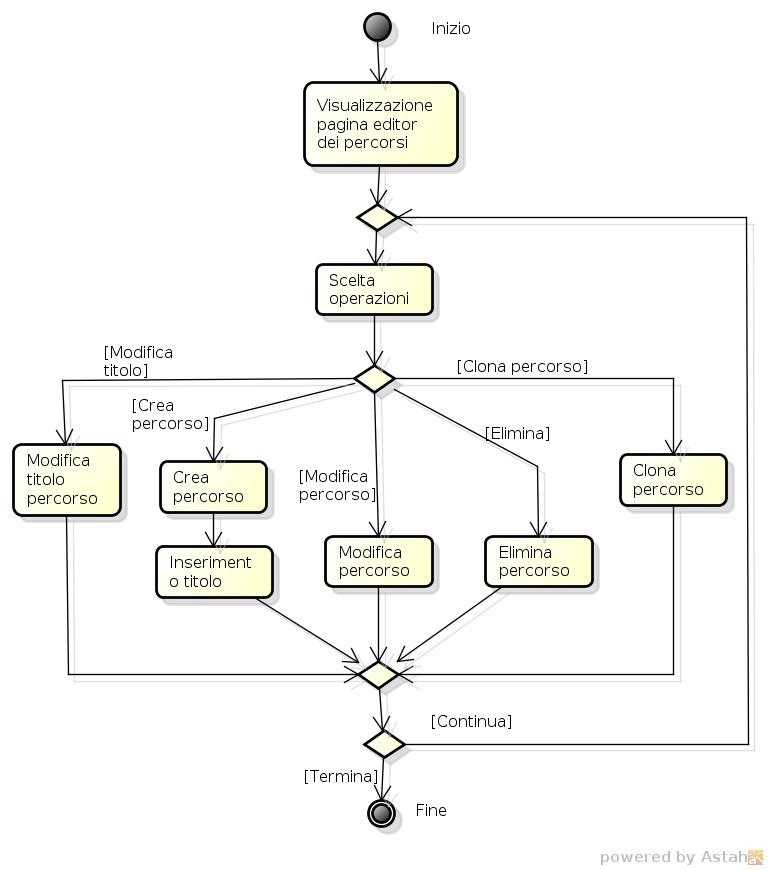
\includegraphics[scale=.5]{img/Editor_percorsi.jpg}
		\caption{Editor percorsi}
		\label{fig:Editor_percorsi}
\end{figure}

Le operazioni che può fare l'utente sono:
\begin{itemize}
\item Modificare il titolo del percorso selezionato;
\item Creare un nuovo percorso inserendo il titolo;
\item Modificare il percorso selezionato;
\item Eliminare il percorso selezionato; 
\item Clonare il percorso selezionato.
\end{itemize}

\newpage

\subsection{Modifica percorso}

\begin{figure}[h!]
		\centering
		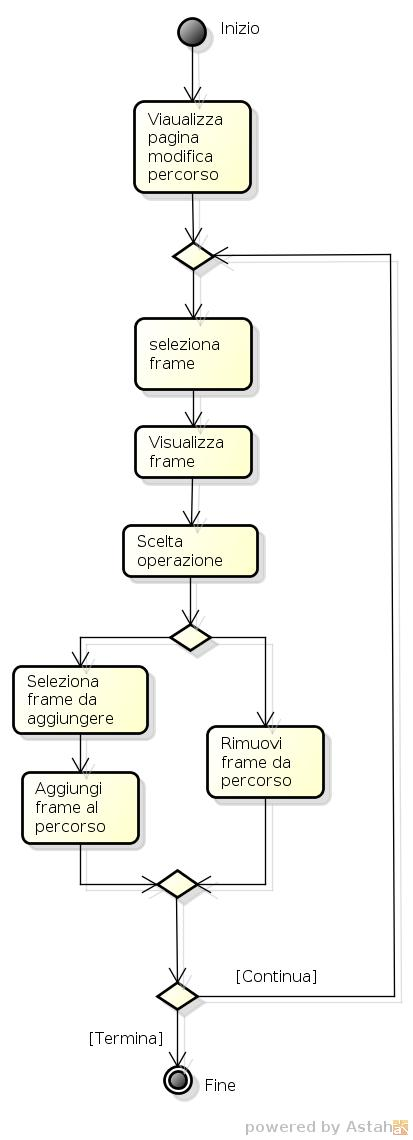
\includegraphics[scale=.5]{img/Modifica_percorso.jpg}
		\caption{Modifica percorso}
		\label{fig:Modifica_percorso}
\end{figure}

Per modificare il percorso l'utente seleziona un frame e questo viene visualizzato nell'editor. Dopodicchè ha la possibilità di rimuovere il frame dal percorso o di selezionarne uno da aggiungerlo al percorso.

\newpage

\subsection{Aggiungi frame}

\begin{figure}[h!]
		\centering
		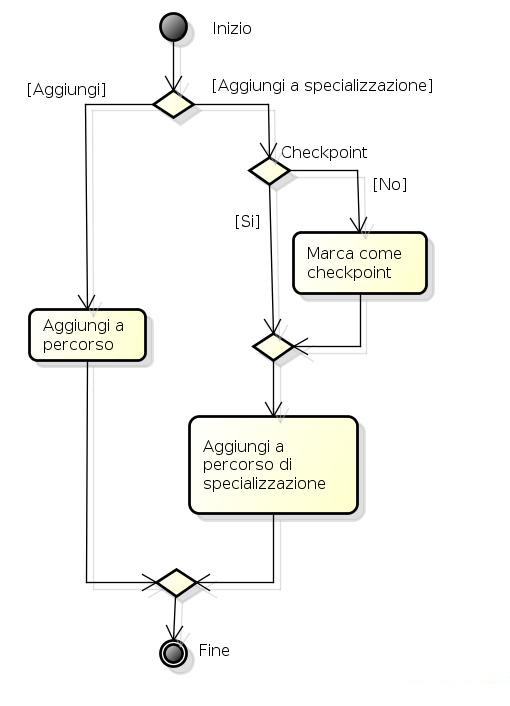
\includegraphics[scale=.5]{img/Aggiungi_frame_al_percorso.jpg}
		\caption{Aggiungi frame}
		\label{fig:Aggiungi_frame}
\end{figure}

Per aggiungere un frame al percorso si hanno due possibilità:
\begin{itemize}
\item Aggiungere il frame in coda al frame visualizzato nell'editor;
\item Marcare il frame corrente visualizzato come checkpoint, se non già marcato, e aggiungerlo al percorso di specializzazione.  
\end{itemize}

\newpage

\subsection{Rimuovi frame da percorso}

\begin{figure}[h!]
		\centering
		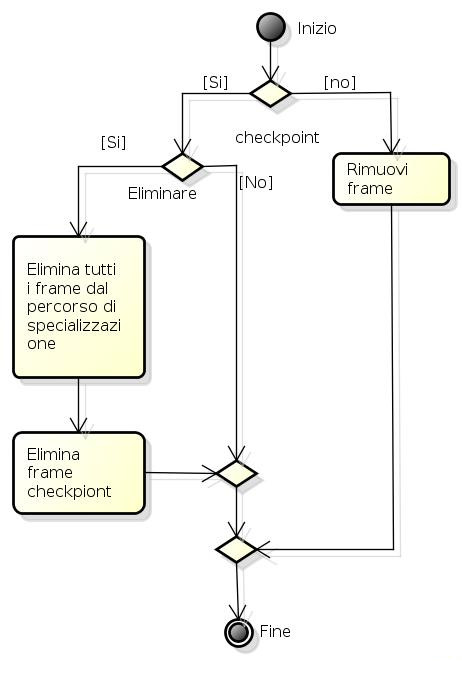
\includegraphics[scale=.5]{img/Rimuovi_frame_da_percorso.jpg}
		\caption{Rimuovi frame dal percorso}
		\label{fig:Rimuovi_frame_da_percorso}
\end{figure}

Quando l'utente rimuove un frame viene controllato se è un checkpoint. In caso negativo si rimuove il frame dal percorso, viceversa se c'è la conferma dell'utente si eliminano prima tutti i frame del percorso di specializzazione e successivamente si elimina il frame dal percorso. 
